\section{ Beacons}  
\label{sec:beacon}  
  
  
\subsection{Communication protocol}  
\label{sec:commprot}  
  
  
The used technology on the beacons was Bluetooth low energy, which has already been introduced on Section \ref{sec:indoortech}. For better understanding the beacon-smartphone communication, it is fundamental to comprehend how this technology works. All the presented information on \ac{BLE} was obtained from its core manual \cite{BLECore}.  
  
 
 
The smartphone and the beacon are set up as two complementary classes. The beacon is defined as a peripheral, a role used to describe devices optimized to support a single connection. This role allows it to have a reduced complexity, since it's only required to function as a slave, an entity that is only capable of receiving connections. On the other hand, the smartphone is defined by the complementary role, central. A central device is capable of supporting multiple connections and is responsible for initiating all of them.  
  
  
 
 
  
  
Another important aspect in understanding this technology is the \ac{BLE} profiles. A profile, which can be seen on Figure \ref{fig:profile} defines an hierarchy in which a device's available services are organized. By doing so, a system's profile ends up defining the applications behaviour and data formats, as well as the manner in which data is exchanged. The hierarchy is composed by two parts: Services and Characteristics.  
  
  
\begin{itemize}  
  
  
\item A profile is composed by one or more services. A service is a collection of data and associated behaviours to accomplish a particular function or feature of a device or portions of a device. It can be either primary, which provides primary functionalities of a device, or secondary, providing auxiliary functionalities of a device and being referenced from at least one primary service. A service is composed of characteristics and/or references to other services.  
  
  
\item A Characteristic is a value that is used in a service that has properties and configuration information that describe how the value should be accessed as well as information on how to display the value. A characteristic is defined by its declaration, its properties, its value and may also be defined by its descriptor, which describes the value or permit configuration of  
the server relative to the value.  
\end{itemize}  
  
\begin{figure}[H]  
\centering  
\includegraphics[width=0.5\linewidth]{2.Chapter/profile.png}  
\caption[Gatt-based profile hierarchy]{Gatt-based profile hierarchy}  
\label{fig:profile}  
\end{figure}  
 
 
  
\subsection{\ac{BLE} enable beacons}  
\label{sec:ble-beacon}  
 
 
 
 
The used beacons are Texas Instruments CC2650STK devices which can be visualised in Figure ~\ref{fig:beacon}. Alongside the device, which comes with a pre-installed Bluetooth low energy program capable of giving information on each of its ten sensors through its predefined profiles, there is a texas smartphone application that can connect to a single device and read from its sensors. By using the texas Code Composer Studio (CSS), the predefined \ac{BLE} profile existent on the device could be changed.  
 
 
 \begin{figure} [H] 
\centering  
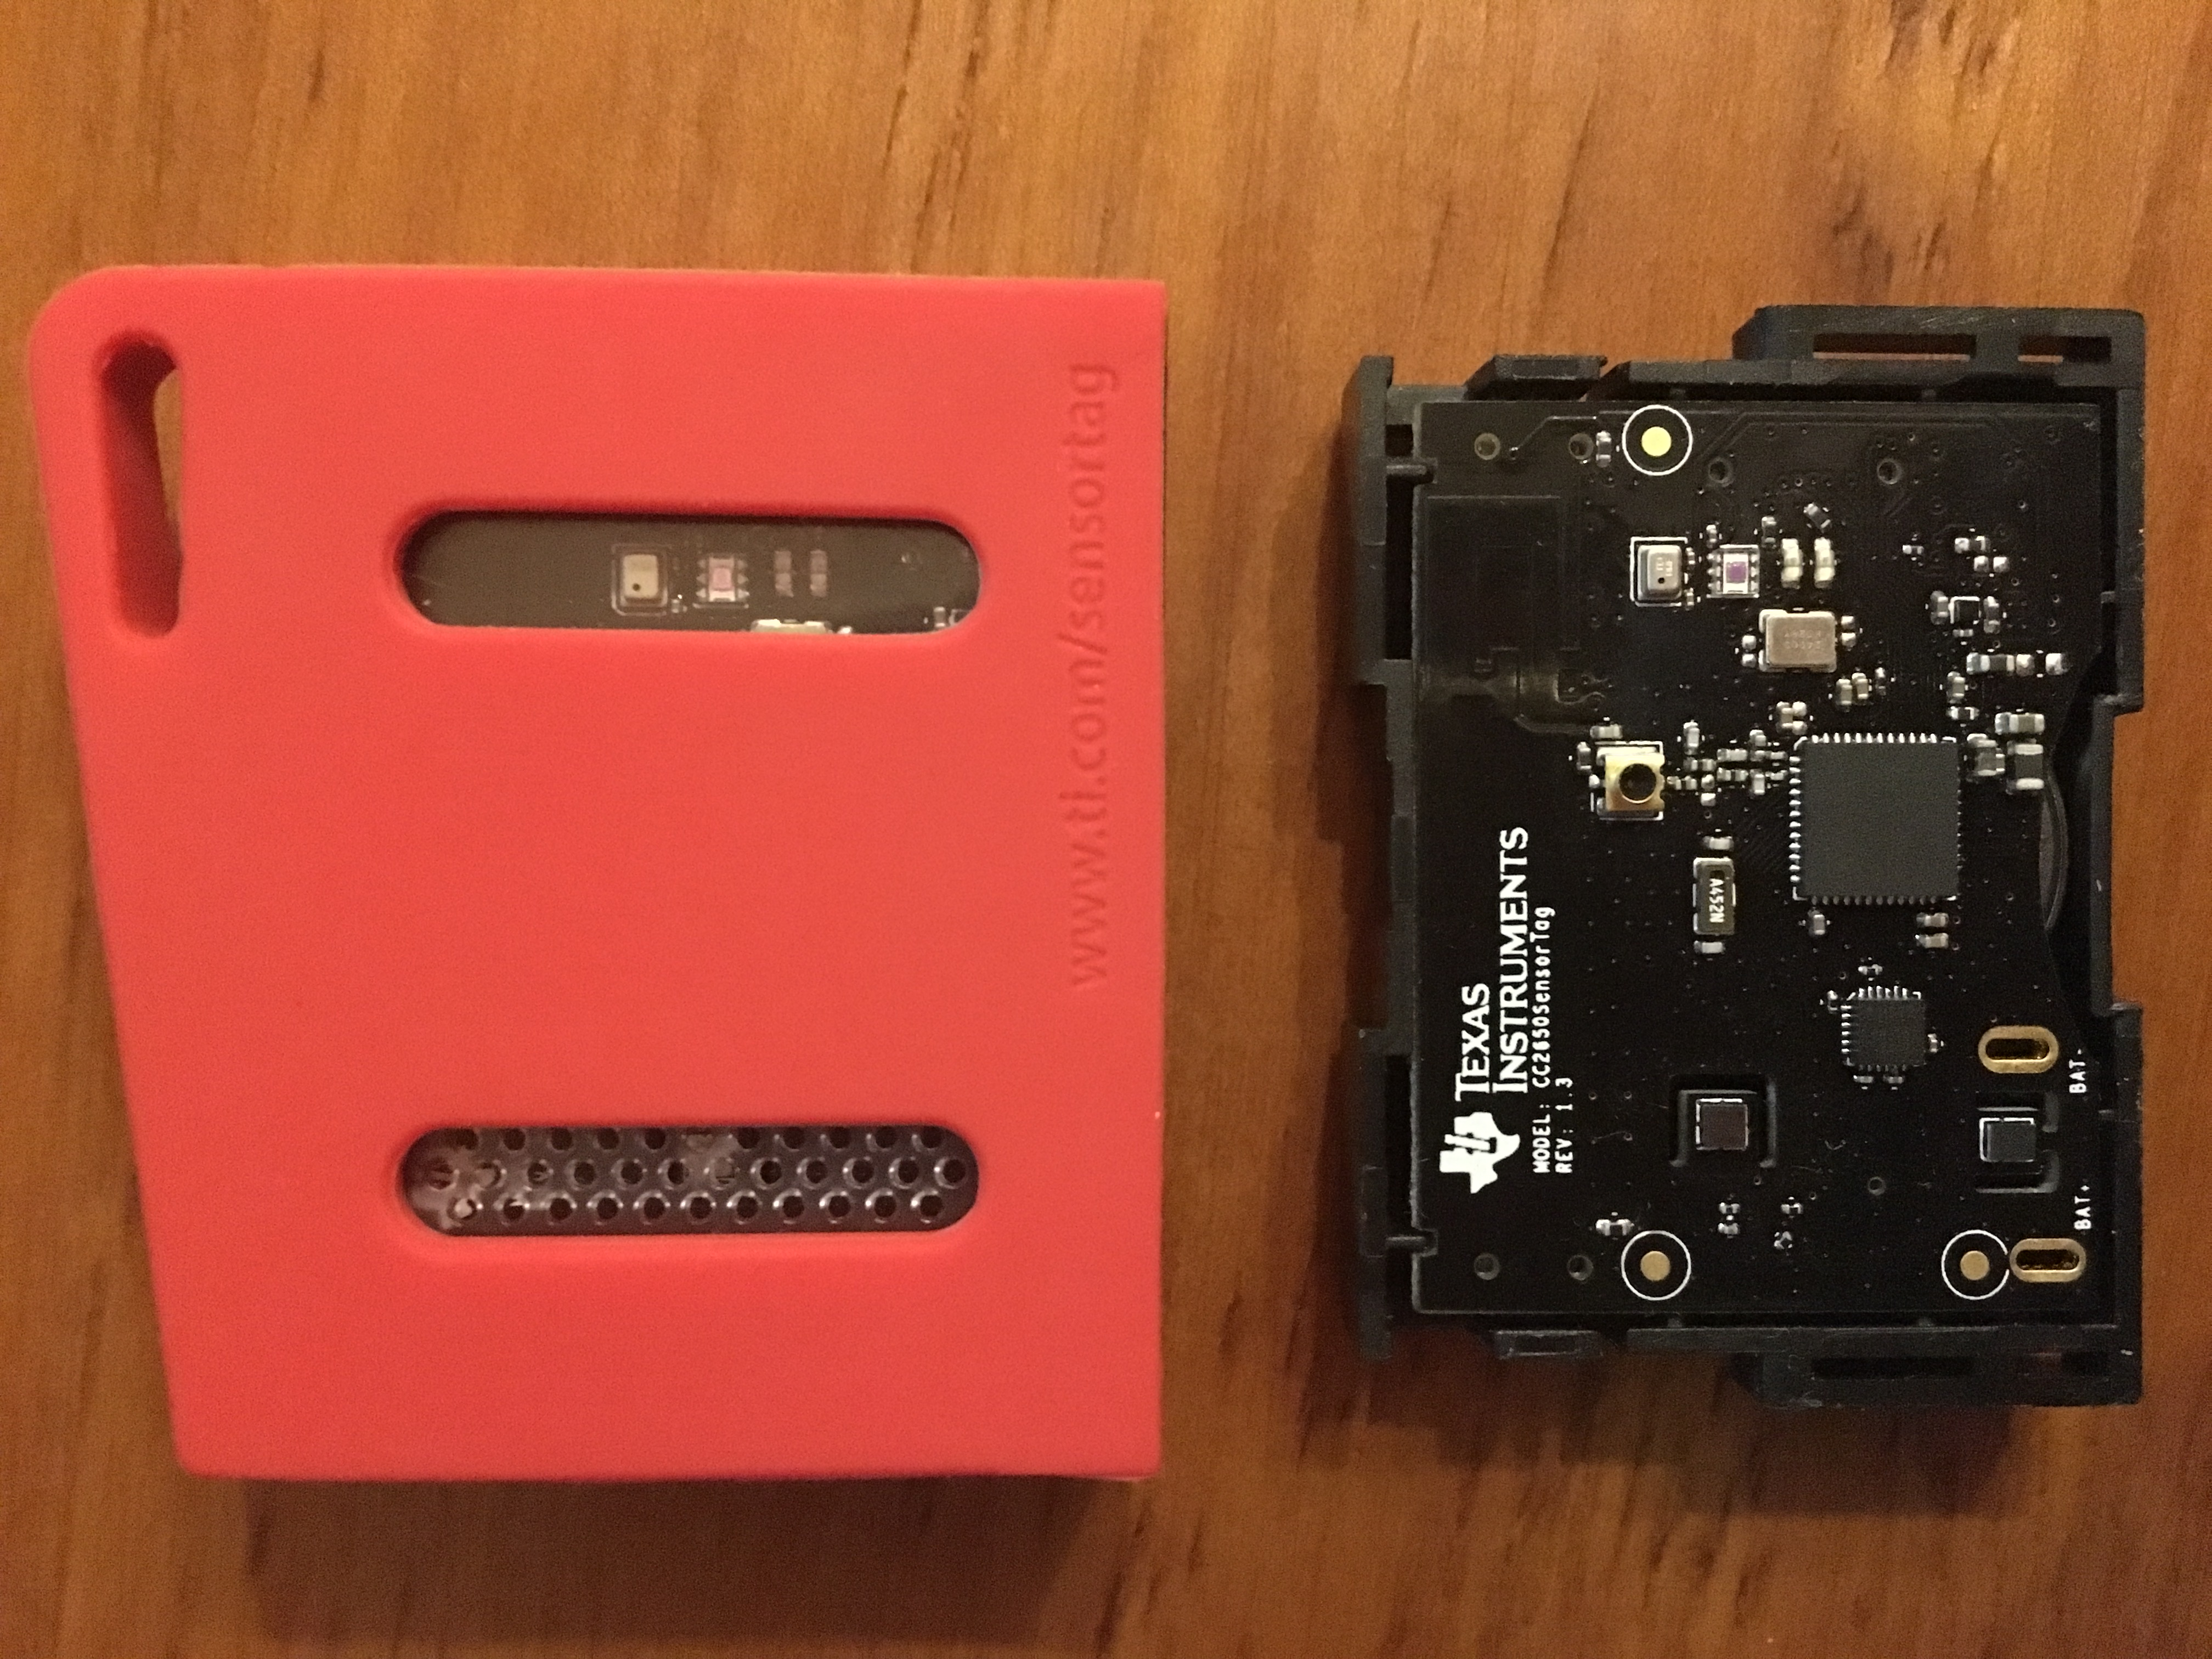
\includegraphics[width=0.5\linewidth]{4.Chapter/beacon.jpg}  
\caption[TI cc2650stk sensortag]{TI cc2650stk sensortag}  
\label{fig:beacon}  
\end{figure}  
 
 
The initial idea was to insert a new service into the already existing profile making use of the generic files provided by Texas.   
In order to implement the service, a characteristic containing the device's server IP and port was created and two random 128-bit universally unique identifier (UUID) were generated. When using UUIDs, the Bluetooth SIG defined several UUID, each associated with a certain service, such as heart rate or glucose services \cite{bleservices}. This situation makes it so that whenever one intends to implements a new service, one has to generate a random 128-bit UUID for his service and another one for each of required characteristics.  
Despite the efforts made, it wasn't possible to alter the existent profile by adding the new service neither by simply attempting to alter it by removing existent services. Due to the low amount of existent information on the technology an alternative was created. The solution found was to store the information into an already functioning service's characteristics as one was capable of altering those kind of parameters. The characteristics available to be used were only the ones from the device information service, a service defined by the Bluetooth sig, since the remaining services on the \ac{BLE} device were meant for reading values of from sensors. The chosen characteristic was the Manufacturer's name due to its low relevance and the fact that its UUID was known, while the remaining's weren't.  
  
 
 
  
In order to reduce the time complexity of the \ac{BLE} communication between the tags and the smartphone application, an attempt was made to reduce the number of connection to a minimum. With the objective of only attempting to communicate with tags that belong to the system while ignoring the remaining, a template name was given to each tag. By adding a common name component, such as \"BLE\_TAG\_SYSTEM\_\" and adding a second part that is device specific, one attempted to apply an initial filter on the nearby \ac{BLE} enabled devices.  
  
  
 
 
  
  
  
 